\chapter{Time-dependent dynamical systems}
Our setup for this chapter will be of nonautonomous $n$-dimensional systems, i.e. the following
\begin{align}
	\dot{x}=f(x,t);\quad x \in \mathbb{R}^{n};\quad t \in \mathbb{R}.
\end{align}
Note that by adding a dimension to our phase space, we can make the system autonomous
\begin{align}
	X =
	\begin{pmatrix}
		x \\ t
	\end{pmatrix}\in \mathbb{R}^{n+1};
	\quad F(X) =
	\begin{pmatrix}
		f \\ 1
	\end{pmatrix}
	\implies
	\dot{X} = F(X).
\end{align}
\section{Nonautonomous linear systems}
For this section, consider
\begin{align}
	\dot{x} = A(t)x + b(t);\quad x \in \mathbb{R}^{n};\quad A(t)\in \mathbb{R}^{n\times n};\quad b(t) \in \mathbb{R}^{n}. \numberthis \label{eq6:star}
\end{align}
We separate \eqref{eq6:star} into two parts. The homogeneous part
\begin{align}
	\dot{x} = A(t)x \numberthis \label{eq6:homo}.
\end{align}
For the homogeneous part we have the solution $x(t) = \Phi_{t_0}^{t}x_0$, for the fundamental matrix solution $\Phi$ with the property $\Phi_{t_0}^{t_0} = I \in \mathbb{R}^{n\times n}$. The inhomogeneous part consists of the rest of \eqref{eq6:star}
\begin{align}
	\dot{x} = b(t).
\end{align}
Thus we find the general solution to \eqref{eq6:star} to be
\begin{align}
	\boxed{
		x(t) = \Phi_{t_0}^{t} x_0 + \Phi_{t_0}^{t}\int_{t_0}^{t} \left( \Phi_{t_0}^{s}\right)^{-1}b(s) ds.
	}
\end{align}
From here we can see that it is enough to understand the homogeneous part. The stability of $x=0$ in \eqref{eq6:homo} is equivalent to the stability of
	$x_p(t) = \Phi_{t_0}^{t}\int_{t_0}^{t} \left( \Phi_{t_0}^{s}\right)^{-1}b(s)ds$
in \eqref{eq6:star}.
Unfortunately the general solution to \eqref{eq6:homo} is unknown.

\section{Time-periodic nonlinear systems}
We now specify our system to be $T$-periodic, thus the evolution rule defined by $\dot{x}=A(t)x$ repeats itself with period $T$, i.e.
\begin{align}
	A(t+T) = A(t).
\end{align}
This implies
\begin{align}
	\Phi_{t_0}^{t-0 +T} = 	\Phi_{t_0+T}^{t-0 +2T} =\Phi_{t_0+2T}^{t-0 +3T} =\ldots =: P_{t_0},  
\end{align}
The operator $P_{t_0}$ is called the \emph{Poincaré map} (or time $T$ map) based at $t_0$. Thus we have
\begin{align}
x_0(t_0+nT) = \underbrace{P_{t_0} \ldots P_{t_0}}_{n  \textrm{ times} } = P_{t_0}^{n}x_0.
\end{align}
The $n$-th iterate of the Poincaré map is denoted by $P_{t_0}^{n}$.

Time being a periodic variable allows us to study the geometry in the extended phase space $\mathbb{R}^{n}\times S^{1}$ as depicted in Fig. \ref{fig:poinc_geom}.
\begin{figure}[h!]
	\centering
	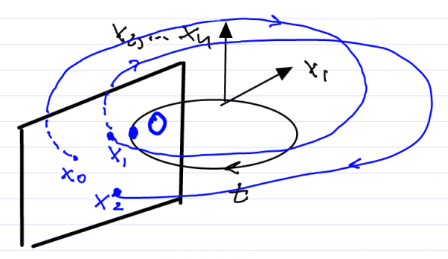
\includegraphics[width=0.5\textwidth]{figures/ch5/1poinc_geom.png}
	\caption{The rectangle represents snapshots of $x$ taken at the interval $T$, thephase space of $x$ is displayed on this plane, while times circles periodically on $S^{1}$. In our snapshots we find $Px_0 = x_1$ and $P^2x_0 = x_2$.}
	\label{fig:poinc_geom}
\end{figure}
Importantly, the stability of $x=0$ can be studied as the stability of the $x=0$ fixed point of the map $P_{t_0}$. Thus we label the eigenvalues of $P_{t_0}$ $\rho_1,\ldots,\rho_n\in\mathbb{C}$  and call these \emph{Floquet multipliers}. We know how to evaluate the stability type of a discrete system such as this, we have two cases
\begin{enumerate}
	\item If there exists an eigenvalue with $|\rho_i|>1$ for $P_{t_0}$ or there exists a repeated eigenvalue with $|\rho_j|=1$ for which the algebraic multiplicity is greater than the geometric multiplicity ($a>g$), then $x=0$ is unstable for \eqref{eq6:homo};
	\item Otherwise, if each eigenvalue of $P_{t_0}$ has magnitude strictly less than 1, i.e. $|\rho_j<1|$, then $x=0$ is asymptotically stable for \eqref{eq6:homo}.
\end{enumerate}

Floquet theory tells us that the following holds in general
\begin{align}
	\boxed{
		\Phi_{t_0}^{t} = {B(t)} e^{\lambda(t-t_0)};\quad B(t+T) = B(t)\in \mathbb{R}^{n\times n};\quad \Lambda \in \mathbb{R}^{n\times n}  \textrm{ is constant} .
	}
\end{align}
\begin{definition}[Floquet exponents]
	The eigenvalues of $\Lambda$ are $\lambda_1,\ldots,\lambda_n\in \mathbb{C}$ are called \emph{Floquet exponents}. We have
	\begin{align}
		\boxed{
			\rho_j = e^{\lambda_j T} = e^{(\alpha_j + i \beta_j)T}.
		}
	\end{align}
	Hence, $\lambda_j$ is well-defined only up to addition of $i2k\pi /T$ for $k \in \mathbb{Z}$. Therefore we have 
	\begin{align}
		|\rho_j| \underset{>}{\overset{<}{=}}1 \Leftrightarrow  \textrm{Re} \lambda _j \overset{<}{\underset{>}{=}} 0.	
	\end{align}
This is generally only numerically computable.	
\end{definition}

We now explore a sufficient criterion for instability of $x=0$. For this we will use Liouville's Theorem (Abel's Theorem)
\begin{align}
	\boxed{
		\det (\Phi_{t_0}^{t}) = \det(\Phi_{t_0}^{t})e^{\int_{t_0}^{t}  \textrm{Tr} \left[ A(s) \right] ds}.
	}
\end{align}
This holds true for any dynamical system $\dot{x}=A(t)x$ with a periodic time-dependence.
\begin{proposition}[Sufficient criterion for instability]
	If we have $\int_{0}^{T}  \textrm{Tr} [A(s)]ds>0$ then $x=0$ is unstable for $\dot{x}=A(t)x$ with $A(t) = A(t+T)$
\end{proposition}
\begin{proof}
Apply Liouville's Theorem to our $T$-periodic system to find
\begin{align}
	\prod_{j=1}^{n} \rho_j = e^{\sum_{j=1}^{n} \lambda_j T} = \det(P_{t_0})	= \det(\Phi_{t_0}^{t_0+T}) = e^{\int_{t_0}^{t_0+T}  \textrm{Tr} \left[ A(s) \right] ds}.	
\end{align}
Now we can compare the arguments of the exponential functions to derive
\begin{align}
	\boxed{
		\sum_{j=1}^{n} \lambda _j = \frac{1}{T} \int_{0}^{T}  \textrm{Tr} \left[A(s) \right] ds.
	}
\end{align}
Therefore our claim holds due to the case differentiation for stability above.  Thus we can verify the stability without the numerical solution of \eqref{eq6:homo}.
\end{proof}
\begin{remark}[]
	The change of variables $x = P(t)y$ transforms the system \eqref{eq6:homo} into the form $\dot{y}=By$, an autonomous linear ODE.
	
	Indeed we obtain that
	\begin{align}
		\dot{y} = P^{-1} (A(t)P - \dot{P})y,
	\end{align}
But
\begin{align}
	\frac{d}{dt}\left( P(t)e^{Bt}\right) = APe^{bt} \implies \dot{P} + PB = AP.
\end{align}
Together this implies $\dot{y} = By$.
\end{remark}
\section{Averaging}
We will now attempt to study the mean evolution of oscillatory systems
\begin{align}
	\dot{x} = f(x,t);\quad x \in \mathbb{R}^{n};\quad f(x,t+T) = f(x,t).
\end{align}
In general the averaged system
\begin{align}
	\dot{y} = \frac{1}{T} \int_{0}^{T} f(y,t)	
\end{align}
does not capture the overall (mean) behavior of the system. This can be demonstrated in an example.
\begin{ex}[Averaging for a swing]
	Mechanically, we examine the stability of a pendulum with a periodically varying length as shown in Fig. \ref{fig:swing_drawing}.
	\begin{figure}[h!]
		\centering
		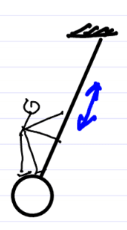
\includegraphics[width=0.1\textwidth]{figures/ch5/2swing_drawing.png}
		\caption{A swing (pendulum) with varying length and a mass $m$.}
		\label{fig:swing_drawing}
	\end{figure}
	The first order model for this system is
	\begin{align}
		\begin{dcases}
			\dot{x}_1 = x_2\\
			\dot{x}_2 = -\omega_0^2 (1+a(t))x_1
		\end{dcases}
		;\quad a(t) = a(t+T),\quad 0<|a|\ll 1.	
	\end{align}
Averaging these equations yields
\begin{align}
	\begin{dcases}
		\dot{x}_1 = x_2 \\
		\dot{x}_2 = -\omega_0^2(1+ \overline{a})x_1.
	\end{dcases}
\end{align}
Where $\overline{a}$ is the average of $a(t)$, a constant. The phase portrait of this is known, as it is just a standard pendulum, i.e. $x=0$ is stable. This means that the small forcing, when averaged, shouldn't move us from the stable position at $x=0$. But we know that by periodically swinging, we don't just stay stuck at the equilibrium point of the swing, and instead begin to swing! Therefore, averaging clearly does not work in this situation.
\end{ex}

However, there are situations in which averaging does work.
\begin{ex}[Averaging in slowly varying periodic systems]
Slowly varying periodic systems are given by
\begin{align}
	\dot{x} = \varepsilon f(x, t, \varepsilon);\quad x \in \mathbb{R}^{n};\quad 0 \leq \varepsilon \ll 1;\quad f(x,t,\varepsilon) = f(x,t+T,\varepsilon).
\end{align}
Such systems are also called \emph{adiabatic} systems.
The averaged system in this case is
\begin{align}
	\dot{y} = \varepsilon \frac{1}{T} \int_{0}^{T} f(y,t,0) = \varepsilon \overline{f_0}(y).	
\end{align}
Here only the leading order terms with respect to $\varepsilon$ in the integrand were taken, as $\epsilon \ll 0$. Now we transform our original equation into the averaged equation via a near-identity change of variables
\begin{align}
	x=y+\varepsilon w(y,t);\quad w(t,t) = w(y, t).
\end{align}
Plugging this transformation into our differential equation, we find
\begin{align}
	\dot{x} &= \left[ I + \varepsilon D_{y}w\right]\dot{y} + \varepsilon \frac{\partial w}{\partial t} \\
	\dot{y} & = \underbrace{\left[ I + \varepsilon D_{y}w \right] ^{-1}}_{I - \varepsilon D_yw + \mathcal{O}(\varepsilon^2)}
	\left[\varepsilon  \underbrace{f(y+\varepsilon w(y,t),t,\varepsilon)}_{=\dot{x}} -\varepsilon \frac{\partial w}{\partial t} \right]\\ 
		&=\varepsilon \left[f(y,t,0) - \frac{\partial w}{\partial t}\right]_{t} + \mathcal{O}(\varepsilon)^2.
\end{align}
In the last equation we used the Taylor expansion. We cannot set $w(y,t) = \int_{0}^{t} f(y,s,0)ds$ as that would be aperiodic. Instead we separate $f$ into two parts, the average and the deviation, $f(y,t,0) = \overline{f}_0 (y) + \tilde{f}(y,t)$. Note that the deviation has mean 0, therefore we set $w(y,t) = \int_{-}^{t} \tilde{f}(y,s)ds$ which is periodic. Therefore we find $\dot{y} = \varepsilon \overline{f}_0(y) + \mathcal{O}(\varepsilon^2)$, noting here that the order 2 term is still $T$ periodic. 

This has given us that the original system is a $T$-periodic, $\mathcal{O}(\varepsilon^2)$ perturbation of the averaged system in the $y$ coordinates. 
\end{ex}

\begin{framed}
	\noindent
	\textbf{Averaging Principle} Solutions of the original equation starting $\mathcal{O}(\varepsilon)$ close to those of the averaged system, stay $\mathcal{O}(\varepsilon)$ close for times of $\mathcal{O}\left(\frac{1}{\varepsilon}\right)$ (very long).
\end{framed}

The averaging principle is depicted in Fig. \ref{fig:avg_principle}.
\begin{figure}[h!]
	\centering
	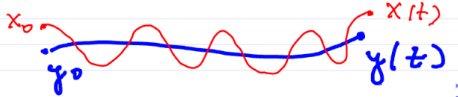
\includegraphics[width=0.7\textwidth]{figures/ch5/3avg_principle.png}
	\caption{For the starting point $x_0$ which is $\mathcal{O}(\varepsilon)$ close to $y_0$, the trajectories remain order $\varepsilon$ close, i.e. $x(t)$ is $\mathcal{O}(\varepsilon)$ close to $y(t)$, for $t \ll \frac{K}{\varepsilon}$.}
	\label{fig:avg_principle}
\end{figure}

This has implications for the Poincaré map of the original equation
\begin{align}
	P_{t_0}^{\varepsilon}:x_0 \mapsto x(t_0+T, x_0; \epsilon);\quad P_{t_0}^{\varepsilon} = P_{t_0}^{0} + \mathcal{O}(\epsilon) \implies \left( P_{t_0}^{\varepsilon}\right)^{n} = \left( P_{t_0}^{0}\right)^{n} + \mathcal{O}(\varepsilon).
\end{align}
This only holds if $n \leq \frac{1}{\varepsilon}$. The time $T$ map of the average system is $P_{t_0}^{0}$.
